\documentclass[11pt,a4paper]{article}
\usepackage[margin=2.2cm]{geometry}
\usepackage[T1]{fontenc}
\usepackage{lmodern}
\usepackage{microtype}
\usepackage{graphicx}
\usepackage{booktabs}
\usepackage{amssymb}
\usepackage{pifont}
\usepackage{xcolor}
\usepackage{caption}
\usepackage{subcaption}
\usepackage{listings}
\usepackage{enumitem}
\usepackage[hidelinks]{hyperref}

\definecolor{okc}{HTML}{0ca30c}
\definecolor{badc}{HTML}{d03b3b}
\definecolor{crc}{HTML}{ec835a}
\newcommand{\cmark}{\textcolor{okc}{\ding{51}}}
\newcommand{\xmark}{\textcolor{badc}{\ding{55}}}
\newcommand{\crash}{\textcolor{crc}{\textbf{!}}}
\lstset{basicstyle=\ttfamily\small,columns=fullflexible,frame=single,framerule=0.3pt}

% generated by scripts/make_figures.py
\newcommand{\DetectionTable}{%
\begin{tabular}{@{}lllllll p{4.2cm}@{}}
\toprule
Vulnerability & \multicolumn{2}{c}{Baseline} & \multicolumn{2}{c}{Hardening} & ASan & MTE-sync / MTE-async & Analysis \\
 & x86 & A64 & x86 & A64 & x86 & A64 & \\
\midrule
Stack buffer overflow & \crash crash & \xmark silent & \cmark canary & \cmark canary & \cmark ASan & \xmark silent / silent & Only stack defenses (canary, ASan) see it; glibc MTE tags heap only \\
Heap buffer overflow & \xmark silent & \xmark silent & \xmark silent & \xmark silent & \cmark ASan & \cmark tag fault / async fault & Spatial: crosses a 16-B granule $\Rightarrow$ MTE detects \\
Out-of-bounds read & \xmark silent & \xmark silent & \xmark silent & \xmark silent & \cmark ASan & \xmark silent / silent & Spatial: lands in granule padding $\Rightarrow$ MTE misses \\
Out-of-bounds write & \xmark silent & \xmark silent & \xmark silent & \xmark silent & \cmark ASan & \xmark silent / silent & Spatial: lands in granule padding $\Rightarrow$ MTE misses \\
Use-after-free & \xmark silent & \xmark silent & \xmark silent & \xmark silent & \cmark ASan & \cmark tag fault / async fault & Temporal: freed memory retagged $\Rightarrow$ MTE detects \\
Double-free & \cmark glibc check & \cmark glibc check & \cmark glibc check & \cmark glibc check & \cmark ASan & \cmark tag fault / async fault & Allocator interaction: glibc tcache check and MTE both catch \\
\midrule
B1 Intra-granule overflow & \xmark silent & \xmark silent & \xmark silent & \xmark silent & \cmark ASan & \xmark silent / silent & Byte-precise ASan vs 16-B MTE granularity \\
B2 Far OOB into live object & \xmark silent & \xmark silent & \xmark silent & \xmark silent & \xmark silent & \cmark tag fault (18/20) / async fault & Jumps ASan redzone; MTE tag mismatch \\
B3 UAF after reallocation & \xmark silent & \xmark silent & \xmark silent & \xmark silent & \xmark silent & \cmark tag fault (19/20) / async fault & ASan quarantine evicted; MTE probabilistic \\
B4 Intra-object overflow & \xmark hijacked & \xmark hijacked & \cmark bounds trap & \cmark bounds trap & \xmark hijacked & \xmark hijacked / hijacked & Inside one object: only index bounds check; CFI territory \\
\bottomrule
\end{tabular}}
\newcommand{\PerfTable}{%
\begin{tabular}{@{}lrrrrrrrrr@{}}
\toprule
 & \multicolumn{3}{c}{x86-64 native: slowdown / RSS} & \multicolumn{6}{c}{AArch64 under QEMU: slowdown (RSS)} \\
\cmidrule(lr){2-4}\cmidrule(l){5-10}
Workload & base (s) & Hard. & ASan & base (s) & Hard. & MTE-sync & & MTE-async & \\
\midrule
alloc-small & 0.51 & 1.01$\times$ & 16.19$\times$ / 24.56$\times$ & 0.46 & 1.00$\times$ & 8.1$\times$ & (1.00) & 8.2$\times$ & (1.00) \\
alloc-medium & 0.74 & 1.00$\times$ & 12.26$\times$ / 19.85$\times$ & 0.47 & 1.00$\times$ & 14.4$\times$ & (1.00) & 14.5$\times$ & (1.00) \\
alloc-large & 0.24 & 0.99$\times$ & 21.50$\times$ / 1.79$\times$ & 0.09 & 1.00$\times$ & 83.1$\times$ & (1.04) & 82.5$\times$ & (1.04) \\
access-seq & 0.50 & 1.09$\times$ & 1.03$\times$ / 1.18$\times$ & 0.16 & 0.99$\times$ & 14.9$\times$ & (1.03) & 14.5$\times$ & (1.03) \\
access-rand & 1.77 & 1.00$\times$ & 1.01$\times$ / 1.22$\times$ & 0.50 & 1.00$\times$ & 1.9$\times$ & (1.02) & 1.9$\times$ & (1.02) \\
kv-store & 1.43 & 0.90$\times$ & 2.07$\times$ / 11.83$\times$ & 1.53 & 1.01$\times$ & 3.5$\times$ & (1.04) & 3.7$\times$ & (1.04) \\
\bottomrule
\end{tabular}}
\newcommand{\CounterTable}{%
\begin{tabular}{@{}lrrrrrr@{}}
\toprule
 & Hard. & \multicolumn{5}{c}{ASan relative to baseline} \\
\cmidrule(l){3-7}
Workload & instr. & instr. & cycles & IPC (base$\to$ASan) & cache-miss & page-faults \\
\midrule
alloc-small & 1.00$\times$ & 20.2$\times$ & 16.0$\times$ & 1.59$\to$2.02 & 1{,}003$\times$ & 1{,}266$\times$ \\
alloc-medium & 1.00$\times$ & 5.0$\times$ & 12.7$\times$ & 1.72$\to$0.68 & 61$\times$ & 158$\times$ \\
alloc-large & 1.00$\times$ & 7.8$\times$ & 21.6$\times$ & 0.83$\to$0.30 & 78$\times$ & 8$\times$ \\
access-seq & 1.00$\times$ & 1.8$\times$ & 1.0$\times$ & 1.04$\to$1.83 & 1$\times$ & 1$\times$ \\
access-rand & 1.00$\times$ & 1.9$\times$ & 1.0$\times$ & 0.03$\to$0.05 & 1$\times$ & 1$\times$ \\
kv-store & 1.02$\times$ & 3.4$\times$ & 2.3$\times$ & 0.83$\to$1.24 & 2$\times$ & 16$\times$ \\
\bottomrule
\end{tabular}}

% generated by scripts/make_figures.py
\newcommand{\ReuseUndet}{12.3}
\newcommand{\ReuseTrials}{40{,}000}
\newcommand{\IrgLagOne}{12.5}
\newcommand{\IrgLagTwo}{7.0}
\newcommand{\HistN}{200{,}000}
\newcommand{\HistMin}{12903}
\newcommand{\HistMax}{13565}
\newcommand{\FarMean}{93.4}
\newcommand{\AdjMin}{85.8}
\newcommand{\AdjMax}{89.1}
\newcommand{\AsanMin}{1.01}
\newcommand{\AsanMax}{21.5}
\newcommand{\AsanRssMin}{1.18}
\newcommand{\AsanRssMax}{24.6}
\newcommand{\AsyncVsSync}{1.01}
\newcommand{\HardInstrMin}{1.00}
\newcommand{\HardInstrMax}{1.02}
\newcommand{\AsanSmallInstr}{20}
\newcommand{\AsanSmallPf}{1{,}266}
\newcommand{\AsanLargePf}{8.2}
\newcommand{\AsanLargeMiss}{78}
\newcommand{\AsanLargeIpc}{0.30}
\newcommand{\BaseLargeIpc}{0.83}
\newcommand{\AsanSeqInstr}{1.77}
\newcommand{\AsanSeqCyc}{1.00}
\newcommand{\AsanRandInstr}{1.91}
\newcommand{\AsanRandCyc}{1.02}
\newcommand{\BaseRandIpc}{0.03}
\newcommand{\AsanKvInstr}{3.4}
\newcommand{\AsanKvPf}{16}


\title{\textbf{Understanding Hardware-Assisted Memory Safety}\\[2pt]
\large An Experimental Study of ARM Memory Tagging and Software Sanitization\\[2pt]
\normalsize Final Project Report --- E0-256 Computer Systems Security}
\author{Suman Roy (SR No: 28164)\\ Indian Institute of Science, Bengaluru}
\date{November 2026}

\begin{document}
\maketitle

\begin{abstract}
This project compares five defense configurations on a common set of C programs with known memory-safety bugs:
an unprotected baseline, compiler hardening, AddressSanitizer (ASan), and ARM's Memory Tagging Extension (MTE) in synchronous and asynchronous mode.
It builds on Noh et al., \emph{ARM MTE Performance in Practice} (USENIX Security 2026).
It reproduces their software configuration: glibc heap tagging is enabled through a tunable on an unmodified binary.
It then extends their evaluation with a detection study, four boundary cases, controlled tag-space experiments and performance profiling.

Against the six-program suite, ASan detects all six violations.
MTE detects three: the heap overflow, the use-after-free and the double-free.
It misses the stack overflow, because glibc tags only heap memory.
It also deterministically misses both out-of-bounds accesses, because they land in the padding of a 16-byte tag granule.
The boundary cases show that the two mechanisms fail on different bugs.
ASan misses a non-linear overflow that jumps into a live object, and a use-after-free whose memory has left its quarantine; MTE catches both about 90\% of the time.
Neither catches an intra-object overflow that hijacks a function pointer.
Only index bounds instrumentation stops that one.

Asynchronous MTE detects the same bugs but reports no fault address and lets the illegal store commit before reporting.
Under QEMU, accidental tag matches after reallocation occur \ReuseUndet\% of the time instead of the ideal 6.7\%.
We trace this to correlated tags from the emulated random-tag instruction (\texttt{IRG}).
Natively, ASan costs \AsanMin--\AsanMax$\times$ in runtime across our workloads.
MTE runtime could only be measured under emulation, so we interpret those numbers against the hardware results of Noh et al.
\end{abstract}

%=====================================================================
\section{Introduction}
Memory-safety violations are still a leading cause of exploitable vulnerabilities in systems software.
Examples are stack and heap buffer overflows, out-of-bounds (OOB) accesses, use-after-free (UAF) and double-free.
Software tools such as AddressSanitizer~\cite{asan} detect many such bugs, but they cost time and memory.
That cost generally confines them to testing.
ARM's Memory Tagging Extension (MTE)~\cite{armmte} offers a different design point.
Each 16-byte granule of memory carries a 4-bit tag, and each pointer carries a 4-bit tag in its top byte.
The hardware checks the two on every access.
Noh et al.~\cite{noh26} recently gave the first comprehensive study of MTE's \emph{performance} on real silicon: Pixel~8/9 cores, AmpereOne and Apple~M5.

This project studies the \emph{security} side of the same trade-off and relates it to performance.
It addresses the four research questions of the proposal:
\begin{enumerate}[label=\textbf{RQ\arabic*},leftmargin=3em,itemsep=1pt]
\item \textbf{Detection coverage:} how does MTE compare with ASan on common spatial and temporal violations?
\item \textbf{Detection boundaries:} which classes are caught by MTE only, by ASan only, or by neither?
\item \textbf{Execution mode trade-offs:} how do synchronous and asynchronous MTE differ in error reporting and performance?
\item \textbf{Security--performance trade-off:} how do runtime and memory overheads compare across allocation-heavy and access-heavy workloads?
\end{enumerate}

\paragraph{Contributions.}
\begin{enumerate}[itemsep=1pt]
\item An evaluation harness for five configurations (Section~\ref{sec:setup}).
It runs one vulnerability suite and records how each run ended: the signal, the \texttt{si\_code} and the source location.
\item A detection matrix (Table~\ref{tab:matrix}) filled from 1{,}400 observed runs, not from assumed guarantees.
\item Four boundary cases that separate byte-precise software checking from probabilistic hardware tagging.
\item Tag-space experiments that measure detection probability against overflow distance and after reallocation.
They expose a tag-generator correlation in emulation.
\item Runtime and memory profiling on allocation-heavy, access-heavy and key-value workloads.
\end{enumerate}

%=====================================================================
\section{Background}
\label{sec:bg}
\paragraph{Compiler hardening.}
\texttt{-fstack-protector-strong} places a random canary between local arrays and the saved return state.
The canary is checked on function return, so the program has already run past the bug when the overflow is detected.
\texttt{\_FORTIFY\_SOURCE} replaces calls such as \texttt{strcpy} with checked variants when the compiler knows the destination size.
\texttt{-fsanitize=bounds-strict} (here with \texttt{-fsanitize-trap}, so it needs no runtime) checks array \emph{indices} against declared array bounds.
These defenses are cheap but cover only narrow patterns.

\paragraph{AddressSanitizer.}
ASan maps every 8 bytes of application memory to one shadow byte.
It surrounds stack, global and heap objects with poisoned \emph{redzones}, and it instruments every load and store with a shadow check.
Freed memory is poisoned and held in a FIFO \emph{quarantine}, 256\,MiB by default on x86-64, before it can be reused.
ASan is deterministic and byte-precise within its model.
That model has two gaps: an access that skips the redzone and lands in another valid object, and a dangling pointer used after its memory has left quarantine.

\paragraph{ARM MTE.}
MTE (Armv8.5-A) associates a 4-bit \emph{allocation tag} with each 16-byte granule.
Bits 56--59 of a pointer hold a \emph{logical tag}, which the Top-Byte-Ignore feature makes possible.
\texttt{IRG} generates a random tag, \texttt{STG}/\texttt{ST2G}/\texttt{DC GVA} write tags to memory, and \texttt{LDG} reads them.
On a mismatch, three reporting modes are available:
\begin{itemize}[itemsep=1pt]
\item \textbf{SYNC} raises a precise \texttt{SIGSEGV} (\texttt{SEGV\_MTESERR}) on the faulting instruction.
\item \textbf{ASYNC} only sets a flag (\texttt{TFSR}), which the kernel turns into \texttt{SEGV\_MTEAERR} at the next kernel entry, with no fault address.
\item \textbf{ASYMM} is synchronous for loads and asynchronous for stores.
\end{itemize}
On Linux, glibc tags heap allocations when the \texttt{glibc.mem.tagging} tunable is set.
Bit~0 enables tagging and bit~1 selects precise (SYNC) faults.
Because MTE relies on random 4-bit tags, it is \emph{probabilistic}: a stale or out-of-bounds pointer goes undetected if its tag happens to match.

\paragraph{Noh et al.~\cite{noh26}.}
The paper evaluates MTE on SPEC CPU and on server workloads (RocksDB, Nginx, PostgreSQL, Memcached).
The binaries are built with Clang~18 and statically linked with glibc~2.36, and MTE is enabled through \texttt{glibc.mem.tagging}.
Overheads are often modest, but every microarchitecture has outliers:
\begin{itemize}[itemsep=1pt]
\item up to 6.64$\times$ on 456.hmmer on the Pixel Performance core in SYNC mode, attributed to store serialization;
\item up to 1.82$\times$ even in ASYNC mode on the Pixel Big core, attributed to a structural hazard on in-flight tag checks;
\item a geometric mean of 1.10$\times$ on AmpereOne in SYNC mode, with 456.hmmer at 1.43$\times$, attributed to store-to-load forwarding.
\end{itemize}
They also show that tagging large allocations, i.e. the cost of \texttt{STG}, is visible on some workloads.
Tagging only allocations below 32\,KiB reduced 403.gcc from 1.23$\times$ to 1.15$\times$ on AmpereOne.
Their artifact (\url{https://github.com/UT-Security/mte-root}) targets MTE hardware: Android Pixel devices and AmpereOne.

%=====================================================================
\section{Experimental Setup}
\label{sec:setup}
\paragraph{Platforms.}
No MTE-capable hardware was available for this project.
The proposal planned for this case: QEMU serves as the functional-validation environment for MTE and is not treated as a substitute for hardware timing.
Two platforms were used:
\begin{itemize}[itemsep=1pt]
\item \textbf{x86-64 native:} AMD Ryzen~5 5600H, Linux, GCC~15.2, glibc~2.43.
It runs Baseline, Hardening and ASan for detection and for real performance numbers.
\item \textbf{AArch64 with MTE:} cross-compiled with \texttt{aarch64-linux-gnu-gcc}~15.2 and run under QEMU~10.2 user-mode emulation with \texttt{-cpu max}, which implements MTE.
It runs Baseline, Hardening, MTE-sync and MTE-async.
\end{itemize}
ASan could not run under QEMU user mode, because its shadow-memory reservation fails, so ASan results come from x86-64.
ASan's checking logic does not depend on the architecture.

Each platform has its own Baseline and Hardening runs, which serve as controls.
The MTE configurations run the \emph{same} AArch64 baseline binary with tagging switched on, so any difference from the AArch64 baseline is caused by MTE alone, not by the architecture or by QEMU.
For the same reason all AArch64 slowdowns are relative to the AArch64 baseline under QEMU, and ASan's are relative to the x86-64 baseline.
Neither platform can replace the other here: ASan, real timings and \texttt{perf} counters exist only on x86-64, and MTE exists only on AArch64.

\paragraph{glibc version.}
The Ubuntu cross sysroot ships glibc~2.43.
With heap tagging enabled, its \texttt{free()} raised a tag-check fault on \emph{every} call, even in a correct \texttt{malloc}/\texttt{free} program.
The fault was a synchronous fault on glibc's own validation load in \texttt{\_\_libc\_free}.
Every MTE result would therefore have been a false positive.
All AArch64 runs instead use Debian~12's glibc~2.36, which is the version Noh et al.\ used.
It is unpacked into a private sysroot and passed to QEMU with \texttt{-L}.
Binaries are compiled with \texttt{-std=gnu17} so that they do not need C23 symbol versions newer than 2.36.

\paragraph{Configurations.}
Table~\ref{tab:configs} lists the five configurations.
Ubuntu's GCC enables stack protection and fortification by default, so the baseline disables them explicitly.
As in Noh et al., MTE needs \emph{no recompilation}: the two MTE configurations execute the baseline binary.

\begin{table}[t]
\centering\footnotesize
\begin{tabular}{@{}lll@{}}
\toprule
Configuration & Build flags / runtime environment & Platform\\
\midrule
Baseline & \texttt{-fno-stack-protector -D\_FORTIFY\_SOURCE=0 -fno-stack-clash-protection} & both\\
Hardening & \texttt{-fstack-protector-strong -D\_FORTIFY\_SOURCE=3} & both\\
 & \texttt{-fsanitize=bounds-strict -fsanitize-trap=all} & \\
ASan & \texttt{-fsanitize=address -fno-omit-frame-pointer}, \texttt{ASAN\_OPTIONS=detect\_leaks=0} & x86-64\\
MTE-sync & baseline binary + \texttt{GLIBC\_TUNABLES=glibc.mem.tagging=3} & AArch64\\
MTE-async & baseline binary + \texttt{GLIBC\_TUNABLES=glibc.mem.tagging=1} & AArch64\\
\bottomrule
\end{tabular}
\caption{Defense configurations. The vulnerability programs are compiled at \texttt{-O0}; the benchmarks at \texttt{-O2}.}
\label{tab:configs}
\end{table}

\paragraph{Optimisation level.}
At \texttt{-O1} and above, GCC deletes most of the suite's bugs.
For example, \texttt{malloc}/\texttt{free}/\texttt{array[0]=42} in \texttt{use\_after\_free.c} folds to nothing, and the never-read \texttt{strcpy} into a dead stack buffer is removed.
Undefined behaviour lets the compiler assume the bug never happens.
The suite is therefore compiled at \texttt{-O0} for \emph{every} configuration, so each defense sees the same faulty accesses.
A consequence is that \texttt{\_FORTIFY\_SOURCE} is inactive in the detection runs, because it needs optimisation.
In a separate check at \texttt{-O2 -fno-builtin}, it caught the heap-buffer \texttt{strcpy} (\texttt{*** buffer overflow detected ***}).

\paragraph{Harness.}
A small \texttt{fault\_reporter.c} is linked into every program, so the suite sources stay unchanged.
It installs \texttt{SA\_SIGINFO} handlers and prints the signal, the \texttt{si\_code} (which separates MTE SYNC from ASYNC), the fault address and the PC offset.
A Python runner maps the PC to \texttt{file:line} with \texttt{addr2line}, or to the nearest symbol.
It classifies every run as \emph{detected} (with the mechanism), \emph{crashed} (a segfault that is a side effect, not a report), or \emph{missed} (the program completed).
The classification uses the ASan report, the glibc abort messages and the fault line.
Every (program, configuration) pair was run 20 times, because MTE tags and allocator reuse are random.
Runtime is the median wall-clock time of 5 runs after a warm-up run, and memory is \texttt{ru\_maxrss} from \texttt{wait4}.
On x86-64, Linux \texttt{perf stat} additionally records cycles, instructions, cache references and misses, branch misses and page faults (mean of 5 runs after a warm-up).
\texttt{perf} is not used for the QEMU runs, because there it would count the emulator's own instructions rather than the guest program's.

%=====================================================================
\section{Phase 1: Vulnerability Suite and Boundary Cases}
Table~\ref{tab:suite} lists the programs.
The six suite programs are those from the proposal, and each has a known bug type and location.
The four boundary cases were added for RQ2 and Phase~4.
Each is built so that the defenses \emph{should} disagree on it.

\begin{table}[t]
\centering\small
\begin{tabular}{@{}lp{10.6cm}@{}}
\toprule
Program & Violation\\
\midrule
\texttt{stack\_overflow} & \texttt{strcpy} of 21 bytes into \texttt{char buffer[10]} on the stack\\
\texttt{heap\_overflow} & \texttt{strcpy} of 21 bytes into \texttt{malloc(10)}\\
\texttt{oob\_read} & read \texttt{arr[5]} of \texttt{malloc(5*sizeof(int))} (byte offset 20 of a 20-byte object)\\
\texttt{oob\_write} & write \texttt{arr[5]} of the same allocation\\
\texttt{use\_after\_free} & \texttt{free(array); array[0]=42;}\\
\texttt{double\_free} & \texttt{free(ptr); free(ptr);}\\
\midrule
B1 \texttt{intra\_granule\_overflow} & write byte 12 of \texttt{malloc(10)}: out of bounds, but inside the object's 16-byte granule\\
B2 \texttt{far\_oob\_into\_live\_object} & \texttt{a[idx]} with \texttt{idx} chosen to land inside a second live object \texttt{b}, skipping ASan's redzone\\
B3 \texttt{uaf\_after\_reallocation} & free a chunk, churn 320\,MiB to flush ASan's quarantine, re-allocate 20{,}000 objects (one reuses the chunk), then write through the stale pointer\\
B4 \texttt{intra\_object\_overflow} & overflow \texttt{name[16]} inside a heap \texttt{struct} into its adjacent function pointer, then call it (control-flow hijack)\\
\bottomrule
\end{tabular}
\caption{Vulnerability suite (top) and boundary cases (bottom).}
\label{tab:suite}
\end{table}

%=====================================================================
\section{Results}
\subsection{RQ1: Detection coverage}
\begin{table}[t]
\centering
\resizebox{\textwidth}{!}{\DetectionTable}
\caption{Comparative evaluation matrix (proposal Table~1), filled from 20 runs per cell.
\cmark\ = detected (mechanism), \xmark\ = missed (the program ran to completion), \crash\ = crashed without a report.
A fraction gives the detected runs out of 20 when not all agreed.
For MTE, the left entry is SYNC and the right entry is ASYNC.}
\label{tab:matrix}
\end{table}

Table~\ref{tab:matrix} and Figure~\ref{fig:matrix} summarise all 1{,}400 runs.

\paragraph{Baseline.}
Without protection, five of the six suite bugs execute silently and the program prints ``Done.''.
The exception is the double-free.
glibc's tcache already detects it (\texttt{free(): double free detected in tcache 2}).
This is an allocator integrity check, not a general memory-safety mechanism.
On x86-64 the stack overflow later crashes on \texttt{ret} (\texttt{SEGV\_MAPERR}), because the saved return address is overwritten.
On AArch64 it runs to completion.
There the link register is saved \emph{below} the locals, so the overflow corrupts the caller's frame instead and the program survives.
The outcome depends on the architecture's frame layout.

\paragraph{Compiler hardening.}
The stack canary detects the stack overflow on both architectures (20/20).
It does so only at function return, \emph{after} the overflowing \texttt{strcpy} and the following \texttt{printf} have executed: ``Done.'' is printed in every run.
Hardening offers nothing for the heap bugs at \texttt{-O0}.

\paragraph{ASan} detects all six suite violations (20/20 each) and reports the exact source line.
It also names the right bug class: \texttt{stack-buffer-overflow}, \texttt{heap-buffer-overflow}, \texttt{heap-use-after-free} and \texttt{attempting double-free}.

\paragraph{MTE} (both modes) detects three of the six suite bugs, each 20/20.
\begin{itemize}[itemsep=1pt]
\item \textbf{The heap overflow}: the 21-byte copy crosses from the 16-byte granule of \texttt{malloc(10)} into the next chunk's header granule.
\item \textbf{The use-after-free}: glibc re-tags freed memory to tag~0, so the stale pointer mismatches.
\item \textbf{The double-free}: the second \texttt{free} performs a tag-checked load inside glibc's \texttt{free}.
\end{itemize}
It misses three:
\begin{itemize}[itemsep=1pt]
\item \textbf{The stack overflow}: glibc's MTE support tags only the heap.
Stack tagging needs compiler support (Clang's \texttt{-fsanitize=memtag-stack}), which GCC~15 does not provide.
\item \textbf{The out-of-bounds read and write}: \texttt{malloc(20)} is rounded up to 32 bytes, i.e. two granules with the same tag.
The access at byte offset~20 lands in the object's own padding, so the tags match.
This miss is \emph{deterministic}, not probabilistic.
\end{itemize}
A bug that is out of bounds for the language can still be in bounds for the tag.
\textbf{MTE's spatial resolution is 16 bytes, not 1 byte.}

\begin{figure}[t]
\centering
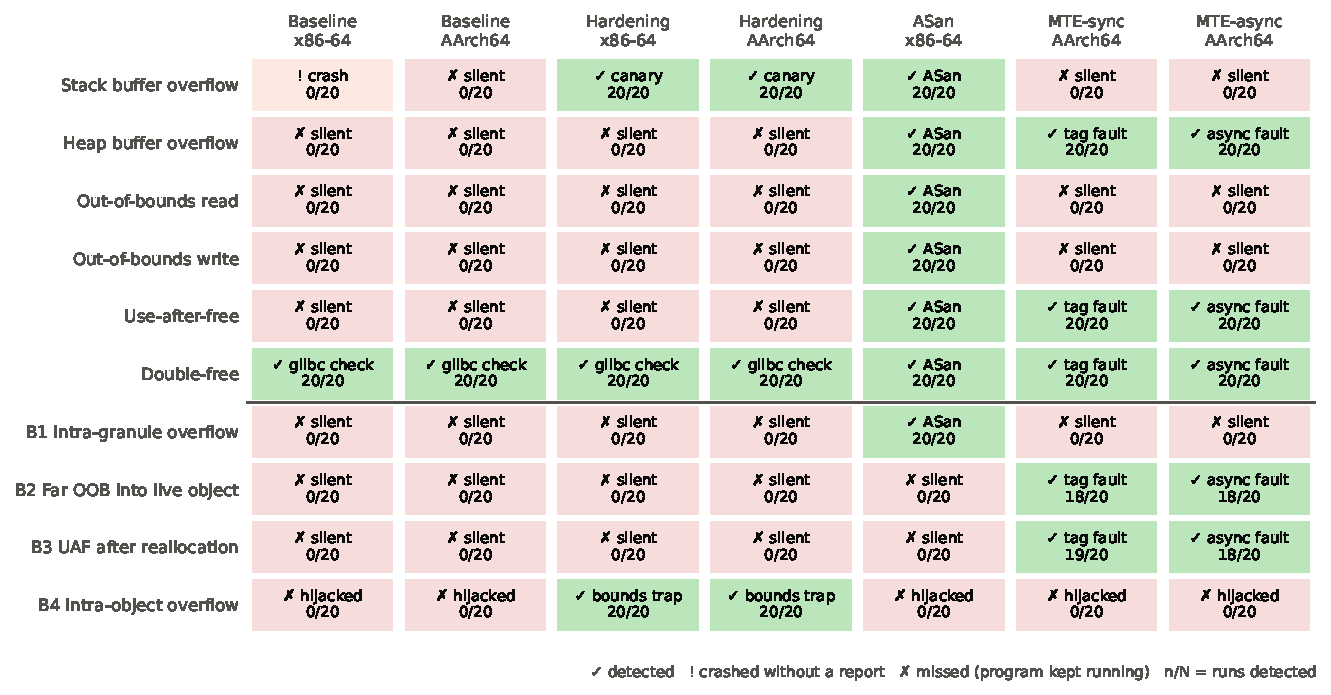
\includegraphics[width=\textwidth]{../figures/detection_matrix.pdf}
\caption{Observed outcome of every program in every configuration (20 runs per cell).}
\label{fig:matrix}
\end{figure}

\subsection{RQ2: Detection boundaries}
The four boundary cases separate the mechanisms cleanly (Table~\ref{tab:matrix}, bottom).
\begin{description}[itemsep=2pt,leftmargin=1.2em]
\item[B1 (intra-granule):]
ASan detects it (20/20), because its shadow encoding records partially addressable 8-byte words.
MTE misses it (0/20) for the granule reason above.
Figure~\ref{fig:granule} measures this boundary directly.
For every request size from 1 to 64 bytes, the first faulting byte offset under MTE is exactly $\lceil n/16\rceil\cdot 16$, in 100\% of the probes.
This leaves up to 15 bytes of undetectable overflow.
ASan detects at offset $n$.
\item[B2 (far OOB into a live object):]
ASan misses it (0/20).
The target address belongs to a valid object, so its shadow is clean.
MTE detects it in 18/20 runs in each mode, because \texttt{a}'s pointer tag differs from \texttt{b}'s memory tag except when they collide by chance.
\item[B3 (UAF after reallocation):]
After 320\,MiB of churn, the freed chunk was reused by a live object in all 20 runs, and ASan reported nothing (0/20).
Its quarantine had been exhausted.
MTE re-tags on every allocation and detects it in 19/20 runs (SYNC) and 18/20 (ASYNC).
The misses are accidental tag matches (Section~\ref{sec:tags}).
\item[B4 (intra-object overflow):]
No baseline, ASan or MTE run detects it.
In every run the overwritten function pointer is called, printing \texttt{CONTROL FLOW HIJACKED}.
ASan places no redzones inside a \texttt{struct}, and MTE tags the whole allocation with one tag.
Only \texttt{-fsanitize=bounds-strict} traps it (20/20), because it knows \texttt{name[]} has 16 elements.
\end{description}
B4 shows that memory tagging is \emph{not} a control-flow defense (course Topic~5).
An attacker who can corrupt a code pointer \emph{within} its own object keeps full control.
That gap is what CFI and pointer authentication are for.

\begin{figure}[t]
\centering
\begin{subfigure}{0.49\textwidth}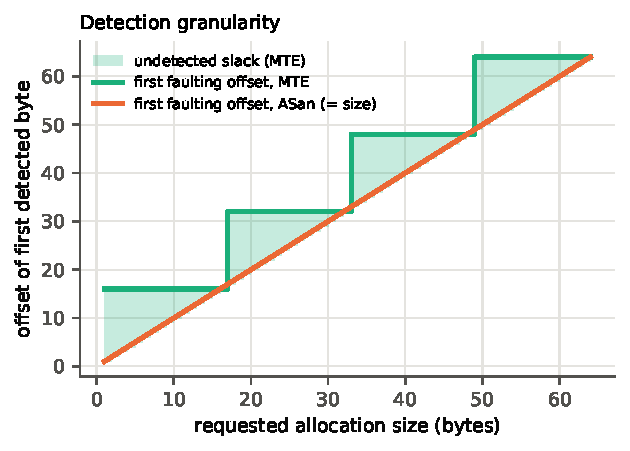
\includegraphics[width=\linewidth]{../figures/granule.pdf}\caption{Detection granularity (MTE-sync vs.\ ASan).}\label{fig:granule}\end{subfigure}\hfill
\begin{subfigure}{0.49\textwidth}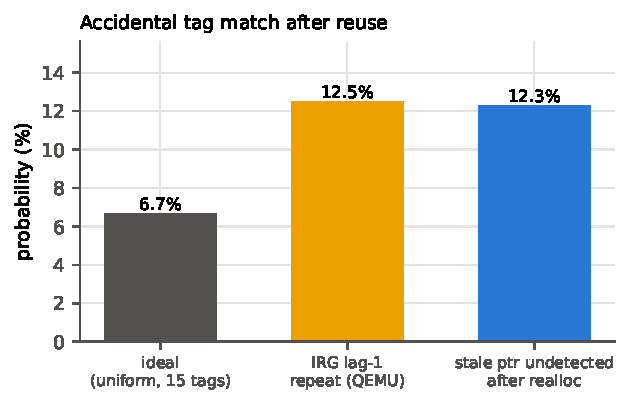
\includegraphics[width=\linewidth]{../figures/tag_reuse.pdf}\caption{Accidental tag match after reuse (\ReuseTrials\ trials).}\label{fig:reuse}\end{subfigure}
\caption{Phase 4: MTE granularity and tag reuse.}
\end{figure}

\subsection{RQ3: Synchronous vs.\ asynchronous MTE}
\label{sec:mode}
\paragraph{Detection.}
On the suite, the two modes detect exactly the same bugs.
The differences are in \emph{what} is reported and \emph{when}.
In ASYNC mode the fault always carries \texttt{si\_addr = 0}.
The PC we recorded is the place where the fault was delivered, not where the bug is.
In the suite it was the next library call after the bug (\texttt{puts@plt}, \texttt{printf@plt}, or glibc's \texttt{free}).
SYNC mode instead points at the source line of the bad access, e.g.\ \texttt{use\_after\_free.c:12}.

\paragraph{Mode probe.}
\texttt{mte\_mode\_probe} performs a single illegal store, or 16 illegal loads, into a neighbouring object that holds a secret.
It then runs a 50-million-iteration loop with no system calls.
Table~\ref{tab:mode} shows the outcome, which was identical in all 10 repetitions.
In SYNC mode the bad instruction never retires: the secret is intact and no leaked byte reaches the program.
In ASYNC mode the illegal store \emph{has already modified the victim object} by the time the fault arrives, and the first leaked byte was already consumed.
QEMU delivers the asynchronous fault at the next translation-block boundary, after at most one loop iteration.
On hardware, Linux delivers it only at the next kernel entry: a system call, an interrupt or a context switch.
The window between corruption and report is therefore \emph{longer} on real hardware than what we observed.
ASYNC therefore detects corruption after the fact rather than preventing it.
It makes exploits unreliable and detectable, but a single committed write may already be enough for an attacker, and the report gives no address for diagnosis.

\begin{table}[t]
\centering\small
\begin{tabular}{@{}llllll@{}}
\toprule
Access & Mode & \texttt{si\_code} & fault address & illegal store committed & leaked bytes used\\
\midrule
store & SYNC & 9 \texttt{SEGV\_MTESERR} & exact (tagged) & no & --\\
store & ASYNC & 8 \texttt{SEGV\_MTEAERR} & \texttt{0} & \textbf{yes} & --\\
load & SYNC & 9 \texttt{SEGV\_MTESERR} & exact (tagged) & -- & 0\\
load & ASYNC & 8 \texttt{SEGV\_MTEAERR} & \texttt{0} & -- & \textbf{1}\\
\bottomrule
\end{tabular}
\caption{Synchronous vs.\ asynchronous reporting (QEMU, 10/10 runs identical).}
\label{tab:mode}
\end{table}

\paragraph{Performance.}
Under emulation, MTE-async runs at \AsyncVsSync$\times$ the time of MTE-sync (geometric mean over workloads).
The two are close because QEMU checks tags in software in both modes.
This does \emph{not} transfer to hardware.
On hardware the modes differ in how the pipeline orders the tag check against the access.
Noh et al.\ found SYNC up to 6.64$\times$ slower on one core, and ASYNC still up to 1.82$\times$ on another, from microarchitectural causes that emulation cannot model.

\subsection{RQ4: Performance and memory overhead}
\label{sec:perf}
\paragraph{Native x86-64 (Figure~\ref{fig:perfx86}, Table~\ref{tab:perf}).}
\emph{Compiler hardening} stays between 0.90$\times$ and 1.09$\times$ of the baseline.
\texttt{perf} shows that these deviations are run-to-run noise: hardening executes \HardInstrMin--\HardInstrMax$\times$ the baseline's instructions.
The benchmarks access memory through pointers, which \texttt{bounds-strict} cannot check, so almost no checks are added.

\emph{ASan's} cost depends strongly on the workload:
\begin{itemize}[itemsep=1pt]
\item \textbf{Allocation-heavy:} 16.2$\times$ (small objects), 12.3$\times$ (1--4\,KiB) and 21.5$\times$ (32--128\,KiB).
Every \texttt{malloc}/\texttt{free} poisons and unpoisons shadow memory, adds redzones and pushes memory through the quarantine.
Peak memory grows by up to 24.6$\times$, because the 256\,MiB quarantine plus redzones dwarf the small live heap.
\item \textbf{Key-value store (mixed):} 2.07$\times$ runtime and 11.8$\times$ peak memory.
\item \textbf{Memory-bound kernels:} ASan costs only 1.03$\times$ on the streaming loop and 1.01$\times$ on the pointer chase.
Its per-access shadow check is hidden behind DRAM bandwidth and latency.
\end{itemize}
ASan's overhead is therefore dominated by \emph{allocator} work and \emph{memory} footprint, not by access checking.

\paragraph{Hardware counters (\texttt{perf stat}, Table~\ref{tab:counters}).}
The counters explain where ASan's time goes:
\begin{itemize}[itemsep=1pt]
\item \textbf{Small allocations:} ASan executes \AsanSmallInstr$\times$ the instructions and causes \AsanSmallPf$\times$ the page faults.
glibc keeps reusing a few hot chunks, while ASan's quarantine keeps handing out fresh memory, so new pages (and their shadow) are touched all the time.
\item \textbf{Large allocations:} the slowdown is larger than the instruction increase, and IPC falls from \BaseLargeIpc{} to \AsanLargeIpc.
Cache misses rise \AsanLargeMiss$\times$: poisoning the shadow and redzones of 32--128\,KiB objects and cycling them through the quarantine is memory traffic, not computation.
\item \textbf{Memory-bound kernels:} ASan executes \AsanSeqInstr$\times$ (streaming) and \AsanRandInstr$\times$ (pointer chase) the instructions, yet cycles change only \AsanSeqCyc$\times$ and \AsanRandCyc$\times$.
The extra shadow-check instructions run in the shadow of DRAM stalls (the pointer chase has an IPC of only \BaseRandIpc), so they are nearly free.
\item \textbf{Key-value store:} \AsanKvInstr$\times$ instructions and \AsanKvPf$\times$ page faults, consistent with a mix of the two cases above.
\end{itemize}
This is the software analogue of the effect Noh et al.\ report for MTE: the cost of a memory-safety mechanism comes mostly from \emph{allocation-time} work and from memory-system effects, rather than from the per-access check itself.

\paragraph{AArch64 under QEMU (Figure~\ref{fig:perfqemu}).}
These numbers are emulation costs: QEMU implements every tag check and every \texttt{STG} in software.
They must not be read as MTE hardware overhead; Noh et al.\ report 1.0--1.43$\times$ on AmpereOne and up to 6.64$\times$ on one Pixel core.
The relative pattern is still informative, because it shows \emph{which} operations MTE adds work to.
Cost rises with the number of bytes tagged per allocation:
\begin{itemize}[itemsep=1pt]
\item 8.1$\times$ for small objects;
\item 14.4$\times$ for 1--4\,KiB objects;
\item 83$\times$ for 32--128\,KiB objects, where glibc must tag the whole object on \texttt{malloc} and re-tag it on \texttt{free}.
\end{itemize}
This is qualitatively the effect Noh et al.\ isolate in their \S4.4.4, where tagging large allocations is expensive and skipping tags above 32\,KiB reduces overhead.
Every access is also tag-checked, so the streaming loop costs 14.9$\times$ in emulation, while the latency-bound pointer chase costs only 1.9$\times$.

Peak RSS grows by 2.3--4.0\% with MTE in every workload, which matches the architectural tag-storage ratio of 4 bits per 16 bytes = 3.125\%.
QEMU allocates that storage for tagged pages; on hardware it is carved out of DRAM and does not show in RSS.
MTE does not inflate the heap the way ASan's redzones and quarantine do: 1.0$\times$ against up to 24.6$\times$.
SYNC and ASYNC are indistinguishable under emulation (Section~\ref{sec:mode}).

\begin{figure}[t]
\centering
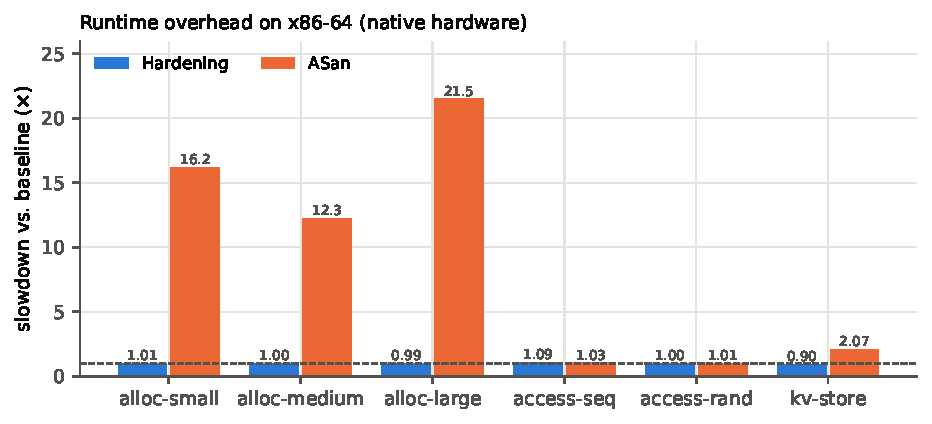
\includegraphics[width=\textwidth]{../figures/perf_x86.pdf}\\[2pt]
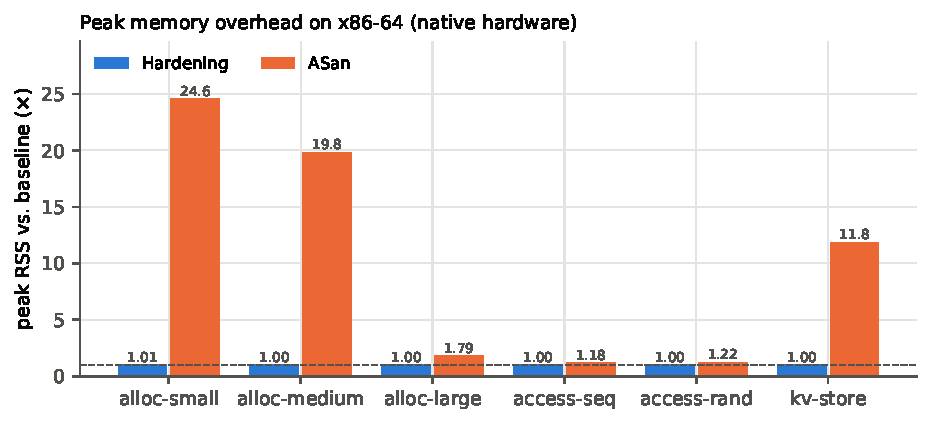
\includegraphics[width=\textwidth]{../figures/perf_x86_rss.pdf}
\caption{Native x86-64: runtime and peak memory relative to the baseline (median of 5 runs).}
\label{fig:perfx86}
\end{figure}

\begin{figure}[t]
\centering
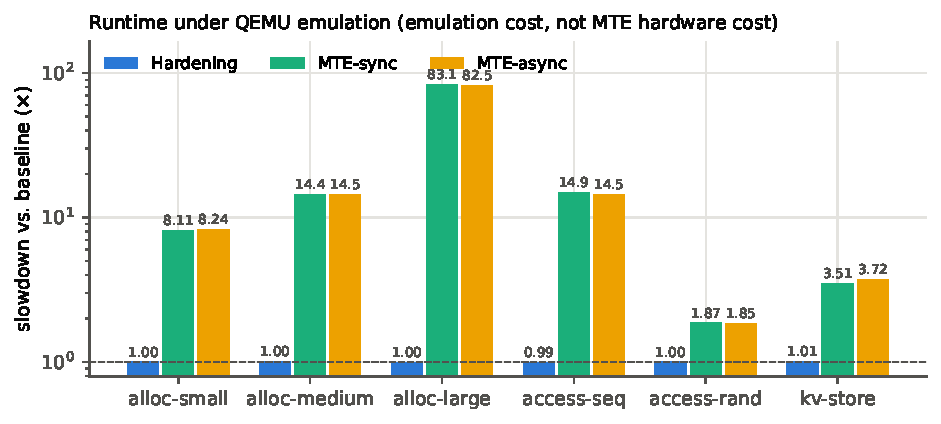
\includegraphics[width=\textwidth]{../figures/perf_qemu.pdf}
\caption{AArch64 under QEMU (log scale). These numbers measure the \emph{emulation} cost of software tag checking and tag setting.
They are not MTE hardware overheads, but they show which operations MTE adds work to.}
\label{fig:perfqemu}
\end{figure}

\begin{table}[t]
\centering
\resizebox{\textwidth}{!}{\PerfTable}
\caption{Median runtime overheads (5 runs). x86-64 shows ``slowdown / peak-RSS ratio'' for ASan. AArch64 RSS ratios are in parentheses and include the QEMU process.}
\label{tab:perf}
\end{table}

\begin{table}[t]
\centering
\small
\CounterTable
\caption{\texttt{perf stat} counters on x86-64 (mean of 5 runs), relative to the baseline. ``Hard.\ instr.'' is the instruction count of compiler hardening; the remaining columns are ASan.}
\label{tab:counters}
\end{table}

\subsection{Phase 4: The finite tag space}
\label{sec:tags}
\texttt{mte\_tag\_space} runs in SYNC mode.
It catches each tag-check fault with \texttt{sigsetjmp}/\texttt{siglongjmp}, so tens of thousands of single-load probes run in one process.
Loads are used so that undetected probes never corrupt the heap.

\paragraph{Tag distribution.}
Across \HistN\ allocations, tag~0 was never handed out, and tags 1--15 occurred between \HistMin\ and \HistMax\ times each, i.e.\ roughly uniformly.
glibc reserves tag~0 for chunk headers and freed memory.

\paragraph{Detection vs.\ distance.}
Figure~\ref{fig:distance} probes an OOB load $d$ bytes past the end of a 48-byte object surrounded by live neighbours.
Each point is 2{,}000 trials, and every object is re-allocated between trials so that all tags are re-randomised.
Three regimes appear:
\begin{itemize}[itemsep=1pt]
\item Every 64 bytes the probe lands on a chunk header (tag~0), and detection is \textbf{100\%}.
\item Elsewhere in far-away objects it averages \textbf{\FarMean\%}, close to the ideal $14/15=93.3\%$.
\item Overflows into the \emph{immediately adjacent} object are detected only \textbf{\AdjMin--\AdjMax\%} of the time.
\end{itemize}
This is the structure the paper summarises as ``a 15/16 chance it will trap''.
Exact numbers depend on the allocator's layout and on tag generation.

\paragraph{Reuse and the tag generator.}
Freed memory is re-tagged to 0, so every stale access \emph{before} reuse was detected (\ReuseTrials/\ReuseTrials).
After the chunk is re-allocated, a stale access goes undetected whenever the new tag equals the old one.
This happened in \textbf{\ReuseUndet\%} of \ReuseTrials\ trials, almost twice the ideal 1/15 = 6.7\% (Figure~\ref{fig:reuse}).
A direct test of \texttt{IRG} explains it.
Under QEMU, two consecutive \texttt{IRG} results are equal with probability \textbf{\IrgLagOne\%}, against 6.7\% for independent tags, while lag-2 results are nearly independent (\IrgLagTwo\%).
A re-allocation and the previous allocation of the same chunk are consecutive \texttt{IRG} calls, and so are two adjacent objects allocated back to back.
This one correlation therefore explains both the reuse rate and the weaker adjacent-object detection above.
\emph{MTE's probabilistic guarantee is only as strong as its tag generator.}
This property must be validated on the actual hardware, and allocators should exclude the previous tag explicitly, as some hardened allocators do~\cite{scudo}.

\begin{figure}[t]
\centering
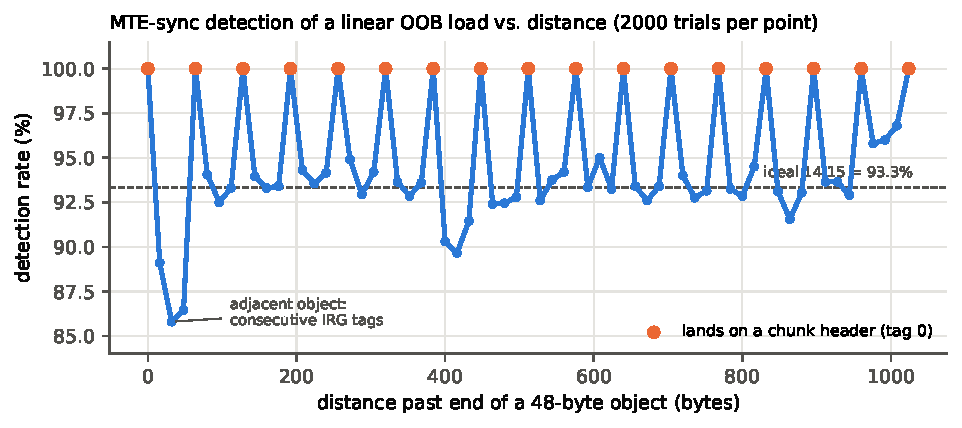
\includegraphics[width=\textwidth]{../figures/tag_distance.pdf}
\caption{Detection probability of an out-of-bounds load as a function of distance (MTE-sync, 2{,}000 trials per point).}
\label{fig:distance}
\end{figure}

%=====================================================================
\section{Discussion}
\paragraph{Security--performance trade-off.}
The mechanisms are complementary, not ranked.
ASan is deterministic and byte-precise near objects, covers the stack, and identifies the bug class.
It cannot see wild accesses that land in valid memory, or use-after-free once memory is reused, and it costs \AsanMin--\AsanMax$\times$ runtime and \AsanRssMin--\AsanRssMax$\times$ memory here.
That keeps it in testing.
MTE needs no recompilation, and its storage cost is fixed by the architecture: 4 bits per 16 bytes, 3.125\%.
It also catches exactly the long-range and temporal cases that ASan misses.
The price is 16-byte granularity, heap-only coverage with glibc and GCC, and probabilistic detection (roughly 88--93\% per access in our measurements).
In ASYNC mode, detection also comes after the corruption.
Noh et al.\ show its hardware runtime cost is usually small but has sharp, microarchitecture-specific cliffs.
Compiler hardening is nearly free but narrow.
Its canary detects stack smashing only at return, and \texttt{bounds-strict} was the only mechanism that stopped the intra-object overflow (B4).

\paragraph{Mapping to the course.}
\begin{itemize}[itemsep=1pt]
\item \textbf{Topics 1--2:} the suite demonstrates stack smashing.
\item \textbf{Topic 3:} the evaluation covers software and hardware defenses.
\item \textbf{Topic 4:} redzones and shadow memory are compared with 16-byte tagging.
\item \textbf{Topic 5:} B4 shows a control-flow hijack that no memory-safety mechanism in our set except index checking prevents.
\item \textbf{Topic 16:} the study exercises MTE instructions, modes and kernel and allocator integration.
\end{itemize}

\paragraph{Limitations.}
\begin{enumerate}[itemsep=1pt]
\item No MTE hardware was available.
MTE detection behaviour is architecturally defined and was validated in QEMU, but MTE \emph{timing} could not be measured.
The \texttt{IRG} correlation may be specific to QEMU.
\item ASan ran on x86-64 rather than AArch64.
\item GCC has no MTE stack tagging, so stack MTE (Clang \texttt{memtag-stack}) is not covered.
\item The suite programs are single-bug micro-programs compiled at \texttt{-O0}, and real code at \texttt{-O2} may behave differently.
\item ASYMM mode was not evaluated.
\end{enumerate}

\section{Conclusion}
On the same programs, AddressSanitizer and ARM MTE catch \emph{different} bugs.
ASan found all six suite violations and the intra-granule overflow, deterministically and with exact diagnostics.
MTE found the heap overflow, the use-after-free and the double-free with no recompilation.
It also found, with roughly 90\% probability, the far-out-of-bounds and reused-memory cases that ASan cannot see.
It missed the stack and every overflow that stays within a 16-byte granule.
Asynchronous MTE detects the same bugs but only after the corrupting access has taken effect, and without an address.
Neither mechanism stops a control-flow hijack through an intra-object overflow.
A deployment that wants low overhead in production should therefore pair MTE with stack protection and control-flow integrity, and should keep ASan for testing.

\begin{thebibliography}{9}\small
\bibitem{noh26} T.~Noh, Y.~Wang, T.~Garfinkel, M.~Madhav, D.~Moghimi, M.~Erez, S.~Narayan. \emph{ARM MTE Performance in Practice}. 35th USENIX Security Symposium, pp.~497--516, 2026.
\bibitem{asan} K.~Serebryany, D.~Bruening, A.~Potapenko, D.~Vyukov. \emph{AddressSanitizer: A Fast Address Sanity Checker}. USENIX ATC, 2012.
\bibitem{armmte} Arm Ltd. \emph{Armv8.5-A Memory Tagging Extension}, white paper, 2019; Arm Architecture Reference Manual for A-profile.
\bibitem{glibc} The GNU C Library Manual, \emph{Memory Related Tunables} (\texttt{glibc.mem.tagging}).
\bibitem{scudo} LLVM Project. \emph{Scudo Hardened Allocator}. \url{https://llvm.org/docs/ScudoHardenedAllocator.html}.
\end{thebibliography}
\end{document}
